\section{Numerical experiments}
\label{sec:exp}
%\begin{figure*}[t!]
%	\begin{center}
%		%\vspace{-0em}
%		\setlength{\tabcolsep}{1pt}
%		\begin{tabular}{ccccc}
%			\rotatebox{90}{$~~~~~~~m=4000$} &
%			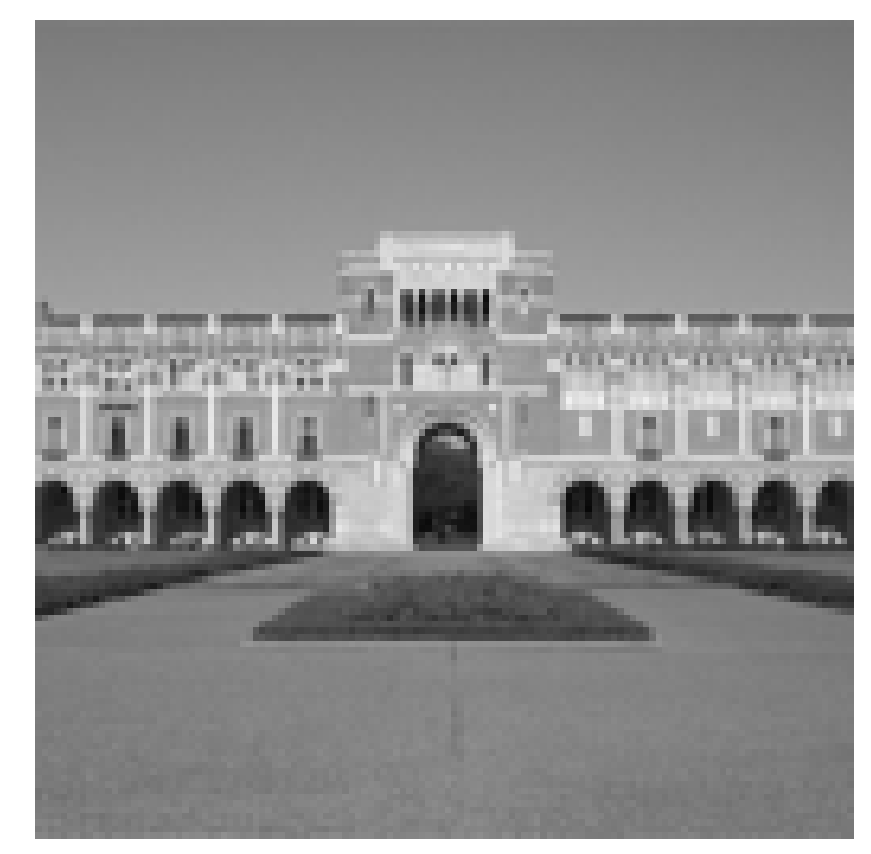
\includegraphics[width=0.22\linewidth]{./fig/lovett_original.pdf} &
%			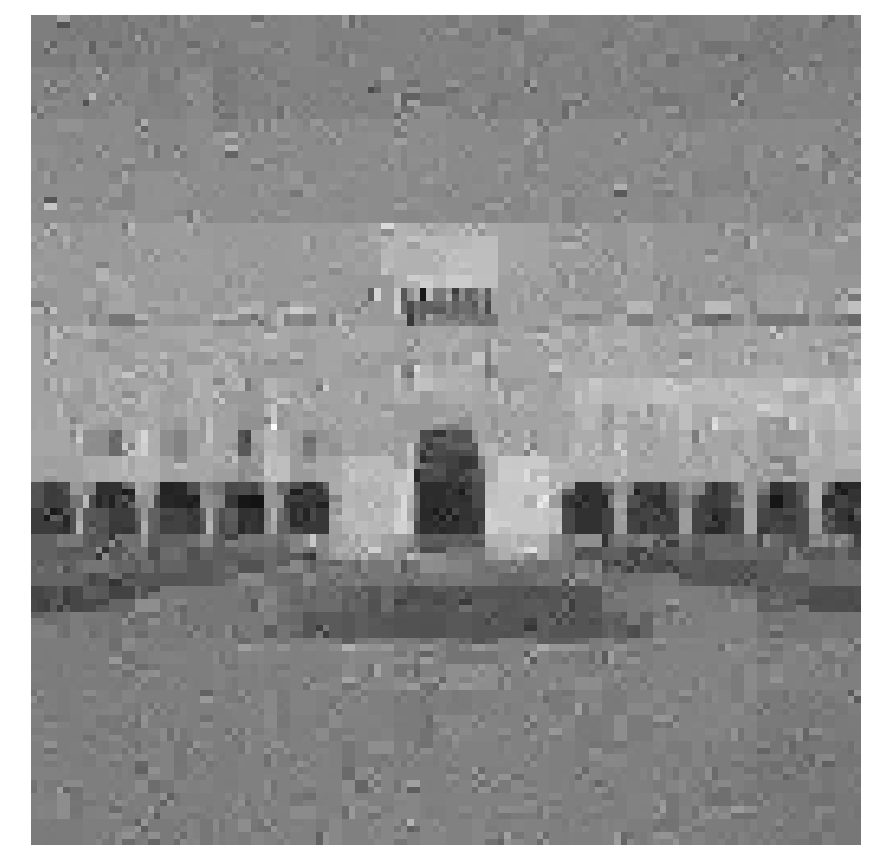
\includegraphics[width=0.22\linewidth]{./fig/lovett_r1_m_4000_s_800.pdf} & 
%			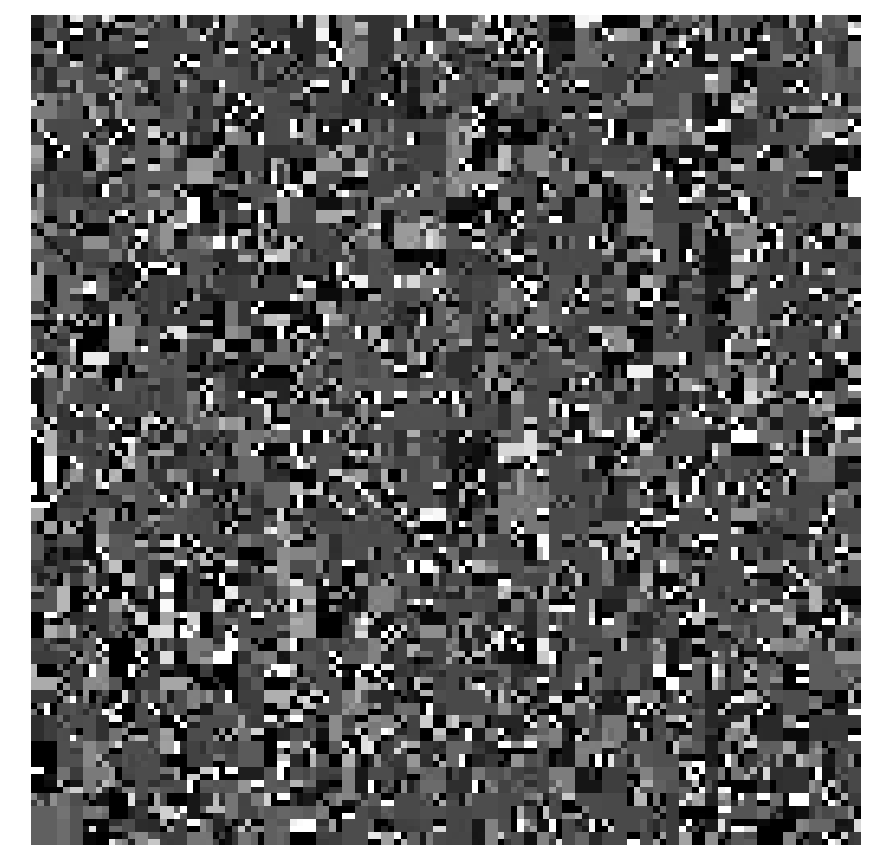
\includegraphics[width=0.22\linewidth]{./fig/lovett_r2_m_4000_s_800.pdf} &
%			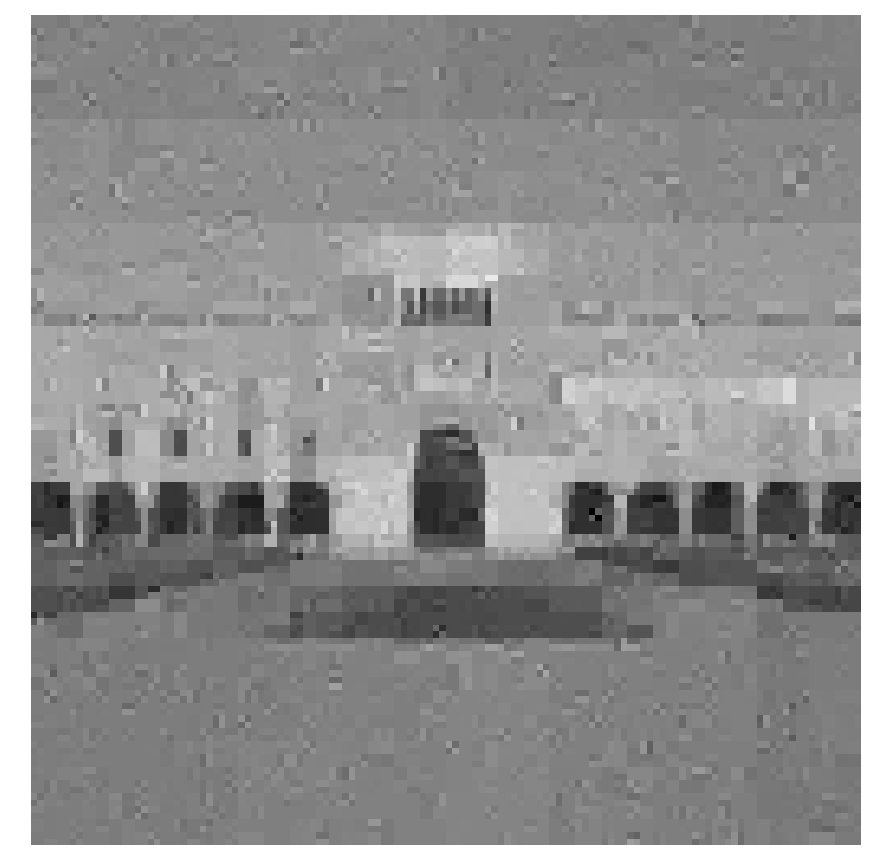
\includegraphics[width=0.22\linewidth]{./fig/lovett_r4_m_4000_s_800.pdf}  \\
%			& \small{(a) Original image}& \small{(b) $R=1$, SNR $=25.06$dB}& \small{(c) $R=2$, SNR $=6.60$dB}& \small{(d) $R=4$, SNR $=26.63$dB} \\
%			
%			\rotatebox{90}{$~~~~~~~m=8000$} &
%			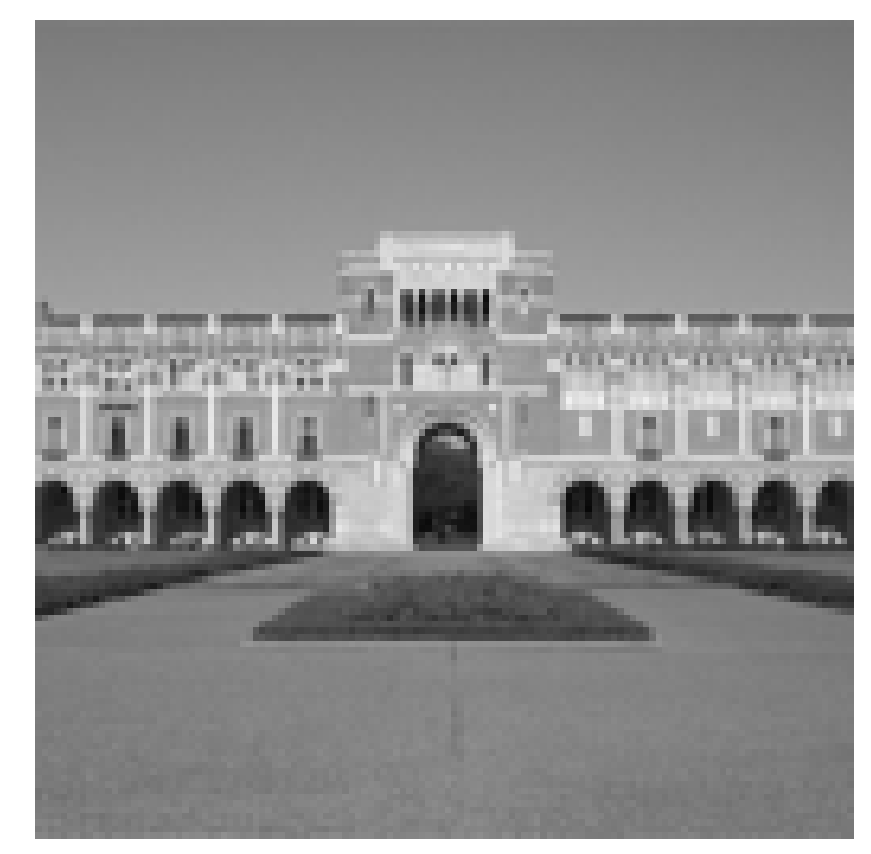
\includegraphics[width=0.22\linewidth]{./fig/lovett_original.pdf} &
%			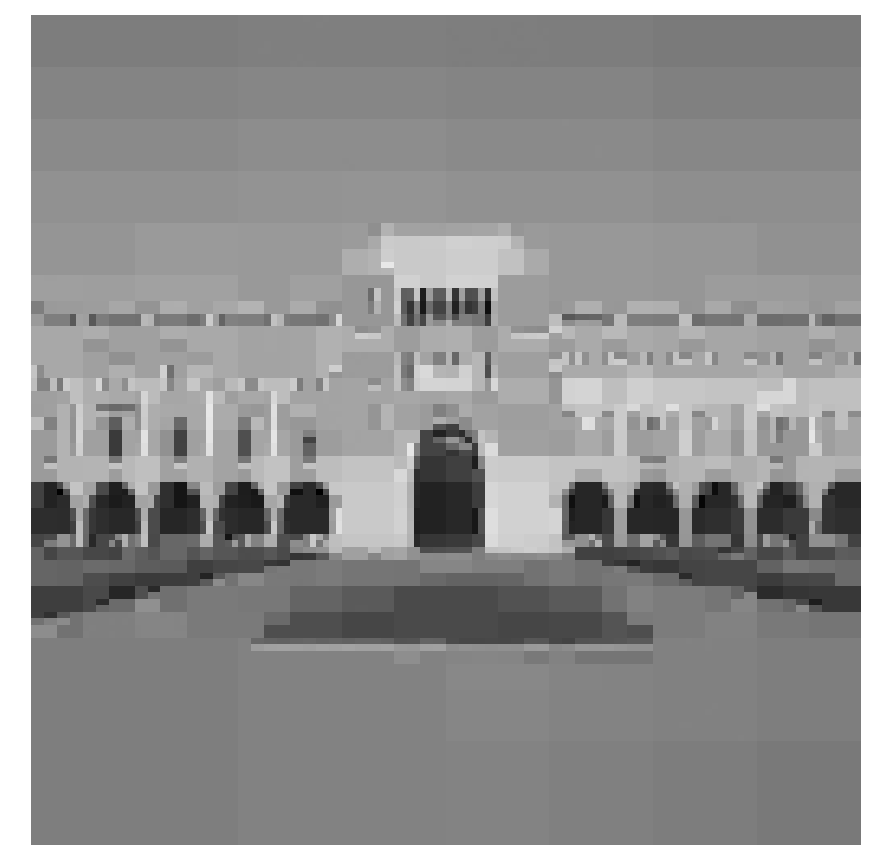
\includegraphics[width=0.22\linewidth]{./fig/lovett_r1_m_8000_s_800.pdf} &
%			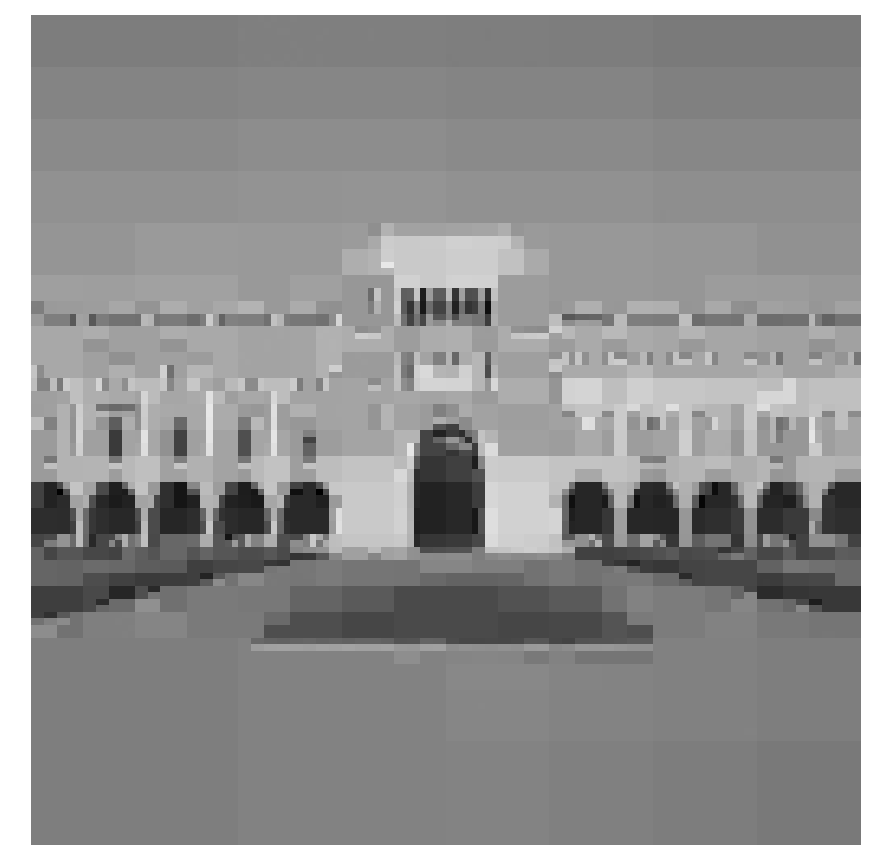
\includegraphics[width=0.22\linewidth]{./fig/lovett_r2_m_8000_s_800.pdf} &
%			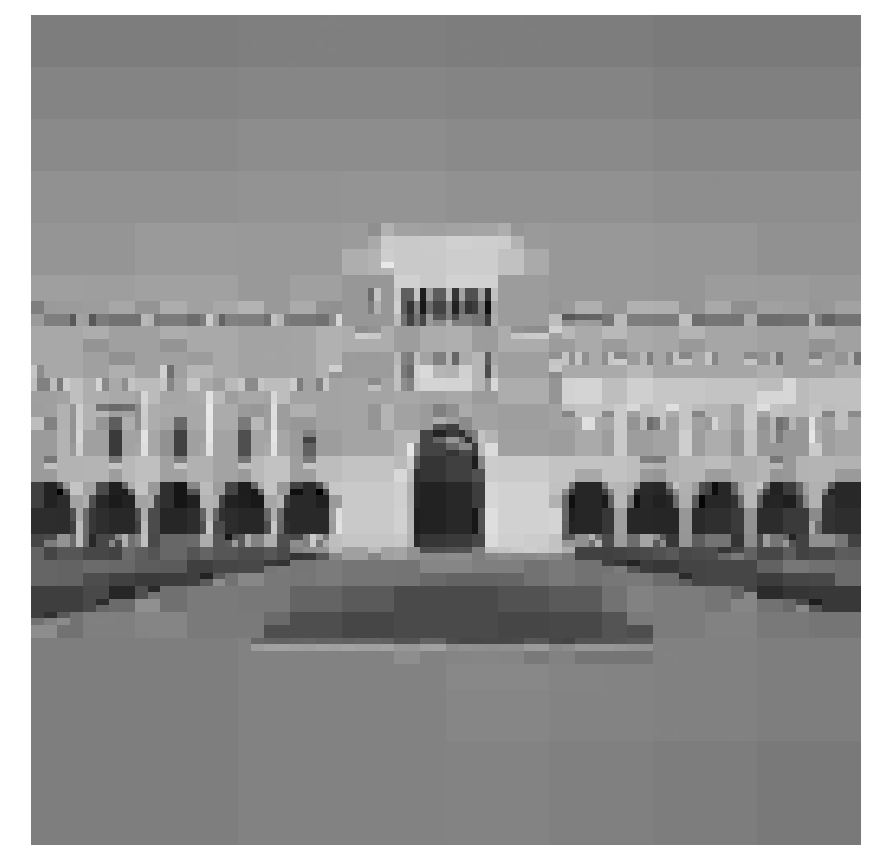
\includegraphics[width=0.22\linewidth]{./fig/lovett_r4_m_8000_s_800.pdf}  \\
%			& \small{(a) Original image}& \small{(b) $R=1$, SNR $=77.71$dB} &\small{ (c) $R=2$, SNR $=76.55$dB} & \small{(d) $R=4$, SNR $=79.29$dB} \\
%		\end{tabular}
%	\end{center}
%	\caption{{(a) Original Lovett Hall image ($n=16,384$); sparse reconstructions ($s=800$) using $m=4000$ (top) and $m=8000$ (bottom) measurements for (b) $R=1$, (c) $R=2$, (d) $R=4$}}
%	\label{fig:lovett}
%\end{figure*}


\begin{figure}[t!]
	\begin{center}
		%\vspace{-0em}
		\setlength{\tabcolsep}{0pt}
		\renewcommand{\arraystretch}{0.5}
		\begin{tabular}{cccc}
			& & $R=4$ & $R=4.5$ \\
			\rotatebox{90}{$~~~~~~~m=4000$} &
			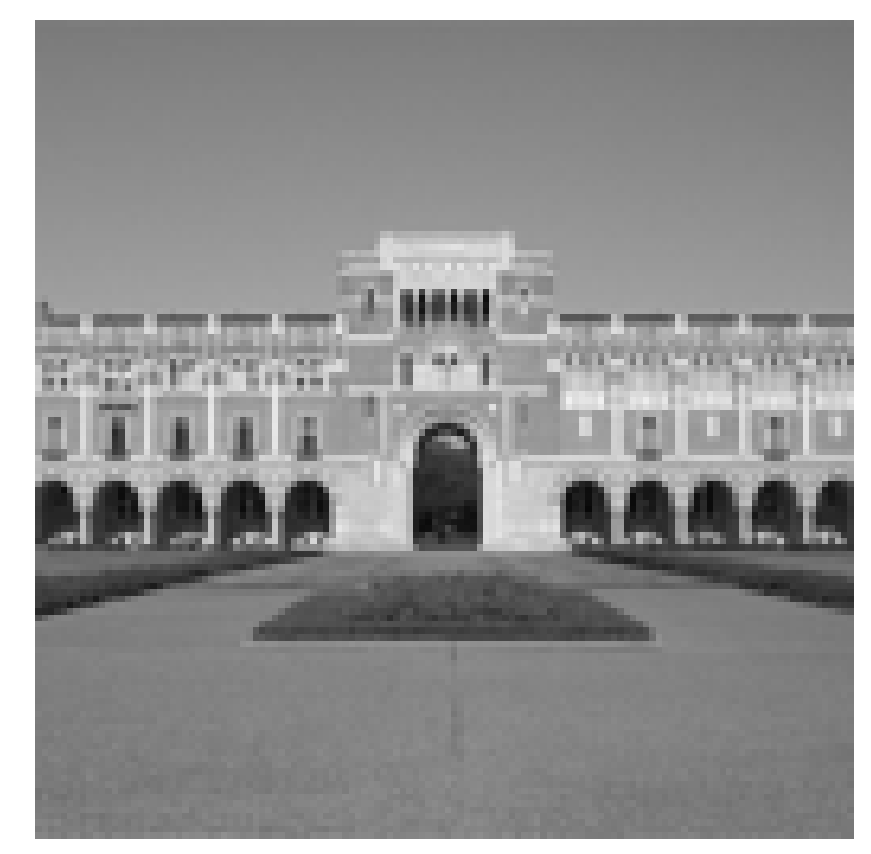
\includegraphics[width=0.32\linewidth]{./fig/lovett_original.pdf} &
			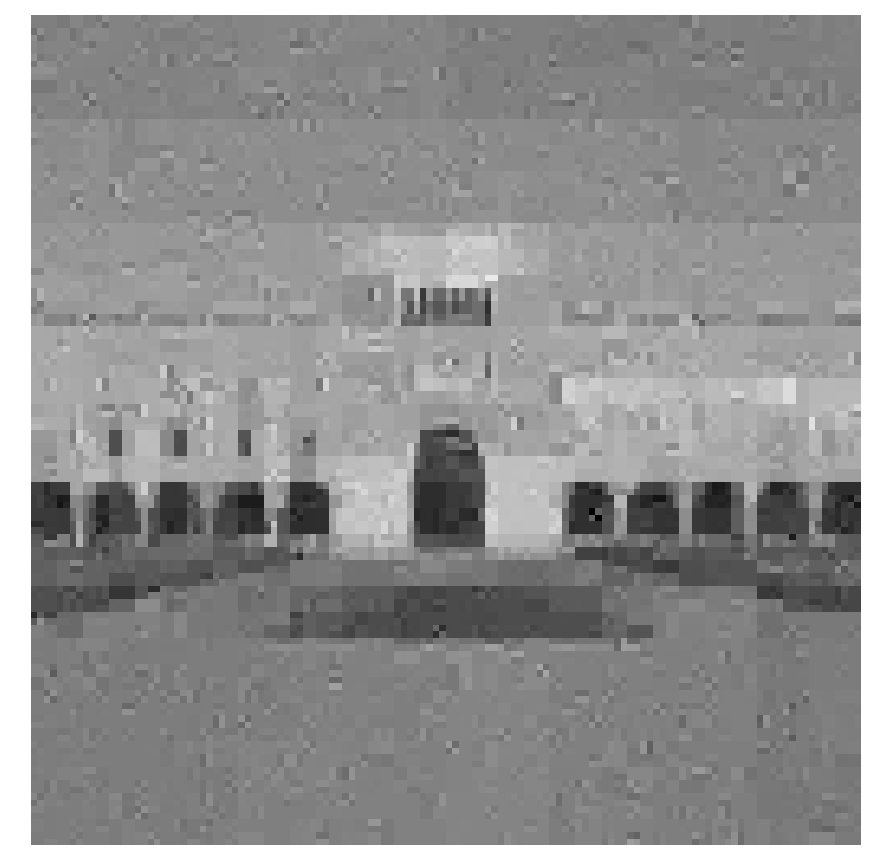
\includegraphics[width=0.32\linewidth]{./fig/lovett_r4_m_4000_s_800.pdf} & 
			%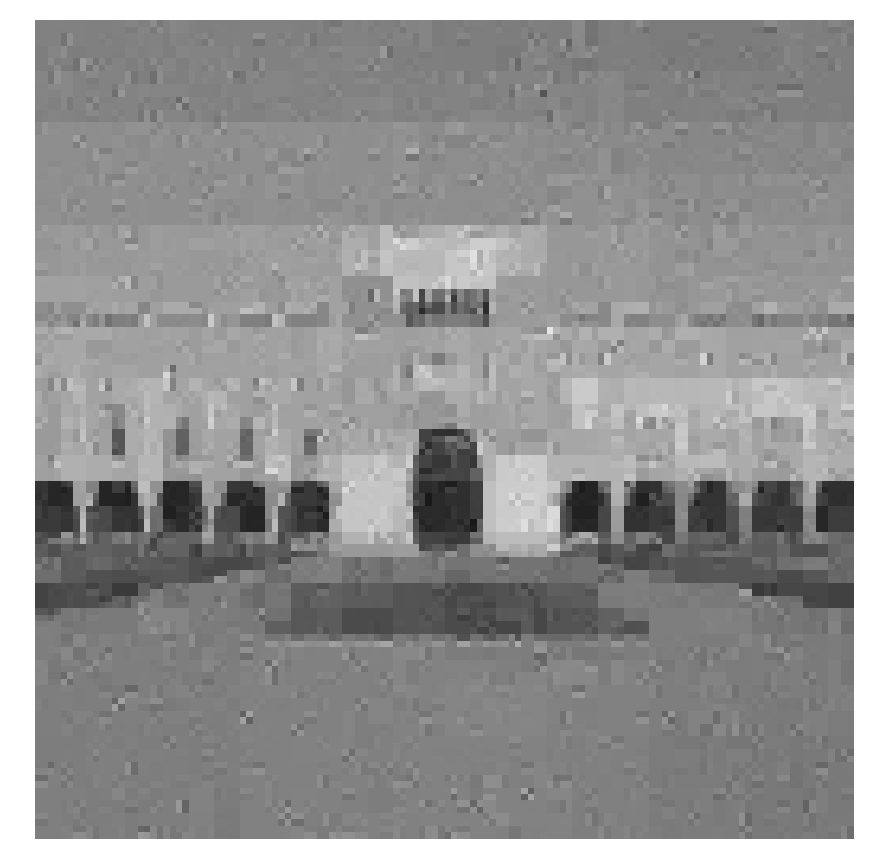
\includegraphics[width=0.22\linewidth]{./fig/lovett_r425_m_4000_s_800.pdf} &
			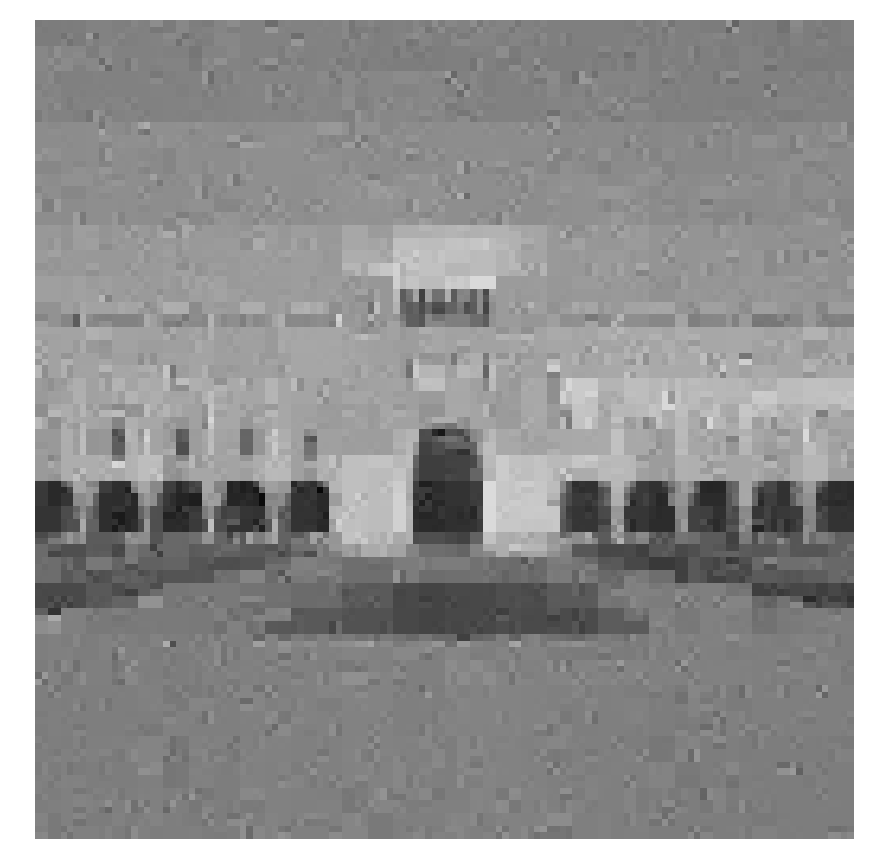
\includegraphics[width=0.32\linewidth]{./fig/lovett_r450_m_4000_s_800.pdf}  \\
			& \small{(a) Original image}& \small{(b) SNR $=26.63$dB}& %\small{(c) $R=4.25$, SNR $=27.20$dB}&
			 \small{(c) SNR $=27.21$dB} \\
			
			\rotatebox{90}{$~~~~~~~m=6000$} &
			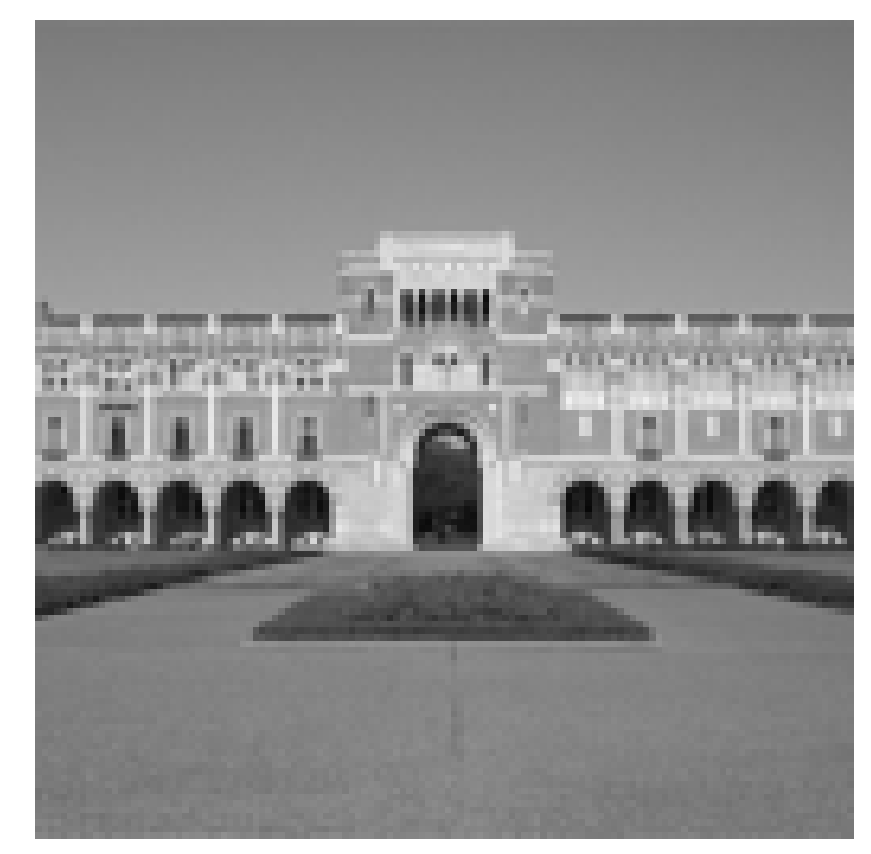
\includegraphics[width=0.32\linewidth]{./fig/lovett_original.pdf} &
			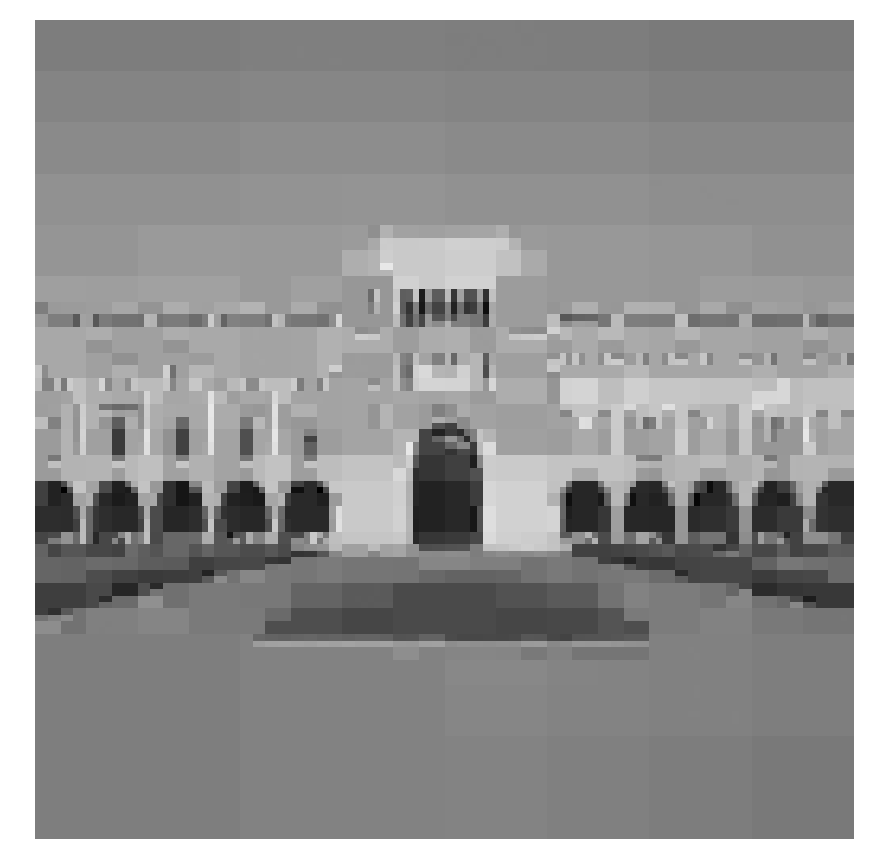
\includegraphics[width=0.32\linewidth]{./fig/lovett_r4_m_6000_s_800.pdf} & 
		%	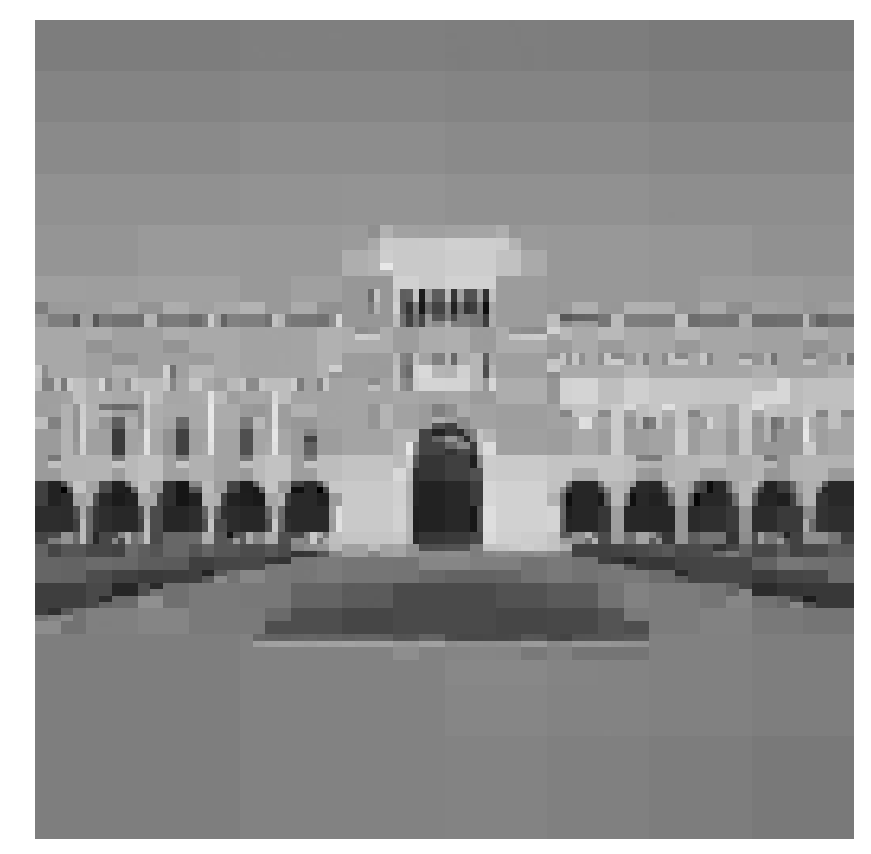
\includegraphics[width=0.22\linewidth]{./fig/lovett_r425_m_6000_s_800.pdf} &
			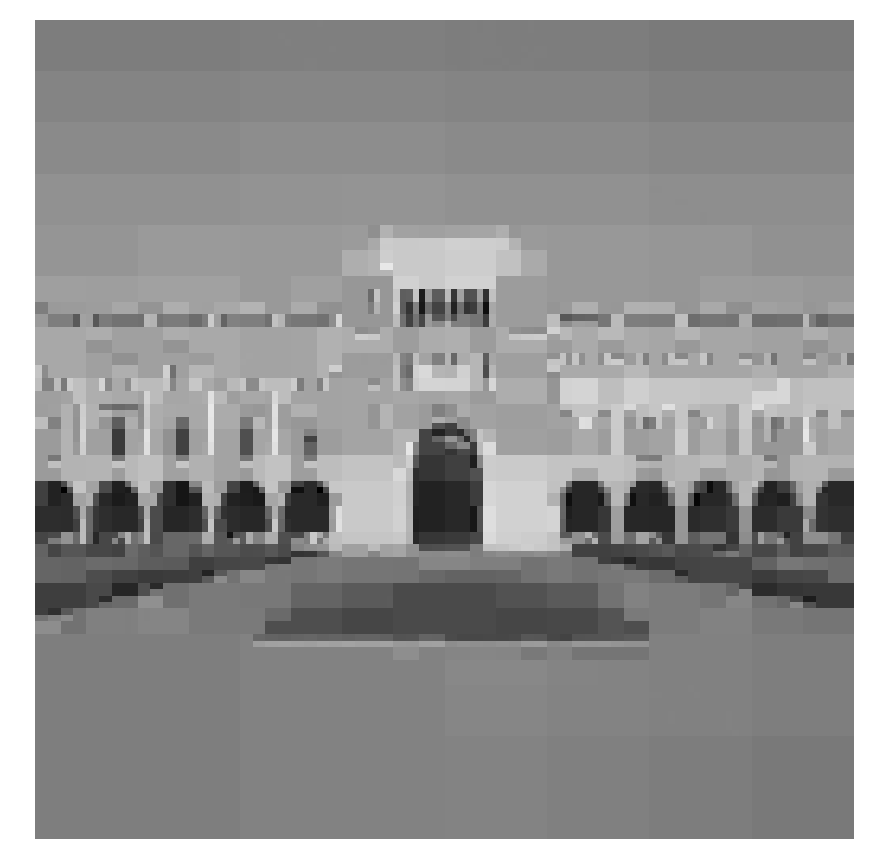
\includegraphics[width=0.32\linewidth]{./fig/lovett_r450_m_6000_s_800.pdf}  \\
			& \small{(a) Original image} & \small{(b) SNR $=81.50$dB} & %\small{(c) $R=4.25$, SNR $=82.88$dB}& 
			\small{(c) SNR $=83.25$dB} \\
		\end{tabular}
	\end{center}
	\caption{{(a) Successful sparse reconstructions ($s=800$) of original Lovett Hall image ($n=16,384$); with $m=4000$ and $m=6000$ measurements for (b) $R=4$, (c) $R=4.5$.}}
	\label{fig:lovett}
\end{figure}

%In this section, we present the results of simulations of signal reconstruction using our algorithm. All numerical experiments were conducted using MATLAB R2017a on a linux system with an Intel CPU and 64GB RAM.
Our experiments explores the performance of the MoRAM algorithm on both synthetic data and real images. We perform experiments on a synthetic sparse signal $\mb{x^*} \in \R^n$ with $n=1000$.The non-zero elements of $\mb{x^*}$ are generated from $\mathcal{N}(0,1)$ and normalized such that $\norm{\mb{x^*}} =1$. The number of measurements $m$ is varied from $m = 100$ to $m=1000$ in steps of $100$. 
%It is important to note that unlike the absolute value function, the modulo function described in Fig.~\ref{fig:compare}(a) is not scale-invariant. The modulo function works over the quantities $y_{c,i}=\langle \mathbf{a_i} \cdot \mathbf{x^*} \rangle, i=1,..,m$; and it is defined over the parameter $R$; thus depending on the magnitudes of $y_{c,i}$ and $R$ relative to each other, the behavior of the measurement model and the reconstruction algorithm would be altered. For instance, if the value of $R$ is too small compared to the range of the $y_{c,i}$, the modulo operation would hardly have any effect on the measurements, leaving $\mathbf{y_c \approx y}$.

%To enforce the quanti, we fix the signal strength by setting $\norm{\mb{x^*}} =1$ in our experiments, while varying the value of modulo parameter $R$ as ${1,2,4}$.

Using $\mb{A, x^*}$ and $\R$, We first obtain the compressed modulo measurements $\mb{y}$ by passing the signal through forward model described by Eq.~\ref{eq:modmeas2}. We reconstruct the signal using MoRAM algorithm and plot the variation of the mean of relative reconstruction error ($\frac{\norm{\mathbf{x^*-x^L}}}{\norm{\mathbf{x^*}}}$) across $10$ such independent experiments vs. number of measurements $m$. In Fig.~\ref{fig:plot} we depict such plots for $2$ values of $R=\{4,4,5\}$ and $4$ values of $s=\{3,6,9,12\}$. It is evident that for each combination of $R$ and $s$, our algorithm converges with probability $1$ to give the exact recovery of the true signal (zero relative error) provided enough number of measurements. In all such cases, the minimum number of measurements required for exact recovery are well below the ambient dimension $(n)$ of the underlying signal. 

%Another important factor affecting the reconstruction is the quality of the initial estimate ($\mathbf{{x}^0}$) obtained through first order estimation. As described in~\ref{sec:init}, the quality of the initial estimate is a direct function of number of measurements ($m$). As we set $m$ higher, the initial estimate $\mathbf{{x}^0}$ would move closer to the original signal $\mathbf{{x}^*}$. For our experiments, we consider two ranges of $m$: $m \in [100,1000]$ and $m \in [1000,10000]$.
\begin{figure}[!t]
	\begin{center}
		\setlength{\tabcolsep}{0pt}
		\renewcommand{\arraystretch}{0.5}
		\begin{tabular}{cc}
			%\vspace{-0em}
			\resizebox{0.5\linewidth}{!}{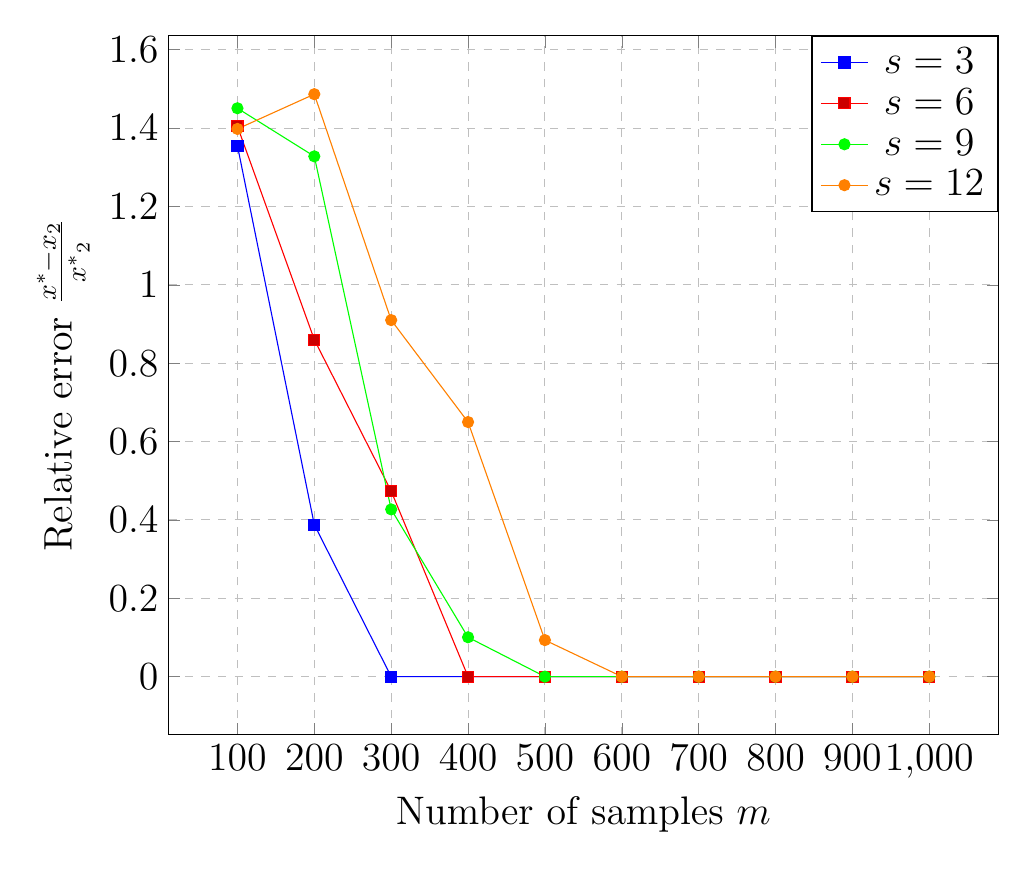
\begin{tikzpicture}
\tikzstyle{every node}=[font=\Large]
\begin{axis}
[width=\linewidth,
xlabel= Number of samples $m$, 
ylabel= Relative error $\frac{\norm{\mb{x^*-x}}_2}{\norm{\mb{x^*}}_2}$,
grid style = dashed,
grid=both,
legend style=
{
at={(1,1), %for arxiv version
%at={(1.65,0.8),  %for NIPS version
anchor=top},
cells={align=center}, 
%legend columns=-1,
} 
]

\addplot[color=blue,mark=square*] plot coordinates {
(100,1.35491249236152)
(200,0.387834861360979)
(300,0.0000838932462760031)
(400,0.0000796709195404289)
(500,0.0000699847485553827)
(600,0.0000654248964096406)
(700,0.0000556622044076941)
(800,0.0000577754338669424)
(900,0.0000476093461140991)
(1000,0.000050430624642886)

};
\addlegendentry{$s=3$};


\addplot plot coordinates {
(100,1.4044226284938)
(200,0.860030446367654)
(300,0.473492899335313)
(400,0.0000833934372627376)
(500,0.0000824008767554939)
(600,0.0000637716674864768)
(700,0.0000644672859553126)
(800,0.0000649831938234799)
(900,0.0000692018122982395)
(1000,0.0000633648746645319)

};

\addlegendentry{$s=6$};


\addplot[color=green,mark=*] plot coordinates {
(100,1.45063072923552)
(200,1.32791017206988)
(300,0.426899433442911)
(400,0.100521404653474)
(500,0.0000847861906819546)
(600,0.0000874052339854557)
(700,0.0000975048393826316)
(800,0.000072296472052776)
(900,0.0000706944130642887)
(1000,0.0000730819848601016)

};
\addlegendentry{$s=9$};

\addplot[color=orange,mark=*] plot coordinates {
(100,1.39786595436235)
(200,1.48655013005159)
(300,0.909955665520478)
(400,0.649802110302209)
(500,0.0932660496014009)
(600,0.0000913091790977068)
(700,0.000104507094662964)
(800,0.0000965628384101342)
(900,0.0000934605996504098)
(1000,0.0000841210242777489)	
};
\addlegendentry{$s=12$};



%\legend{CoPRAM\\Block CoPRAM\\ThWF\\SPARTA\\}

\end{axis}
\end{tikzpicture}} &
			%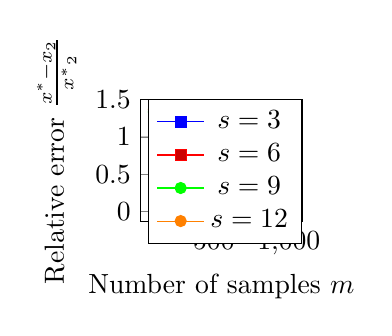
\begin{tikzpicture}
\begin{axis}
[width=0.3\textwidth,
xlabel= Number of samples $m$, 
ylabel= Relative error $\frac{\norm{\mb{x^*-x}}_2}{\norm{\mb{x^*}}_2}$,
grid style = dashed,
grid=both,
legend style=
{
at={(1,1), %for arxiv version
%at={(1.65,0.8),  %for NIPS version
anchor=top},
cells={align=center}, 
%legend columns=-1,
} 
]

\addplot[color=blue,mark=square*] plot coordinates {
	(100,0.747375723427608)
	(200,0.155095058698698)
	(300,0.0000819832015109237)
	(400,0.0000795274009640216)
	(500,0.0000641794969526483)
	(600,0.0000695356190000224)
	(700,0.0000613755178216418)
	(800,0.000066926164718668)
	(900,0.0000621778223230091)
	(1000,0.0000567630039894841)
};
\addlegendentry{$s=3$};


\addplot plot coordinates {
(100,1.27659964262396)
(200,0.43032378497965)
(300,0.0000910097212427942)
(400,0.0000954106153959511)
(500,0.0000809830346078354)
(600,0.0000657018308358537)
(700,0.0000812049368096766)
(800,0.0000603853227824464)
(900,0.000061849877746736)
(1000,0.0000623366305719791)
};

\addlegendentry{$s=6$};


\addplot[color=green,mark=*] plot coordinates {
(100,1.33360297687866)
(200,0.695654696202488)
(300,0.379473134000177)
(400,0.000102603470161568)
(500,0.000103129235494395)
(600,0.0000859751501828087)
(700,0.0000828224635500562)
(800,0.0000879068415403419)
(900,0.0000671510294321006)
(1000,0.0000630635849783938)
};
\addlegendentry{$s=9$};

\addplot[color=orange,mark=*] plot coordinates {
(100,1.36704835741717)
(200,0.932318539564495)
(300,0.559981038525355)
(400,0.000119464801989713)
(500,0.000091109865406022)
(600,0.0000977493433158512)
(700,0.000114550943002834)
(800,0.0000954985216580123)
(900,0.0000848854981296593)
(1000,0.0000637656776977681)
};
\addlegendentry{$s=12$};



%\legend{CoPRAM\\Block CoPRAM\\ThWF\\SPARTA\\}

\end{axis}
\end{tikzpicture} &
			\resizebox{0.45\linewidth}{!}{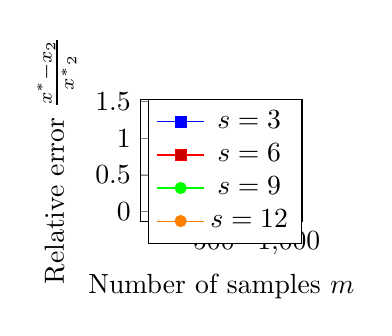
\begin{tikzpicture}
\begin{axis}
[width=0.30\textwidth,
xlabel= Number of samples $m$, 
ylabel= Relative error $\frac{\norm{\mb{x^*-x}}_2}{\norm{\mb{x^*}}_2}$,
grid style = dashed,
grid=both,
legend style=
{
	at={(1,1), %for arxiv version
		%at={(1.65,0.8),  %for NIPS version
		anchor=top},
	cells={align=center}, 
	%legend columns=-1,
} 
]

\addplot[color=blue,mark=square*] plot coordinates {
(100,0.577929457493856)
(200,0.0000837291793747255)
(300,0.0000793871859744244)
(400,0.0000727181866723273)
(500,0.0000754214852024106)
(600,0.0000687961736114565)
(700,0.0000623167482713836)
(800,0.0000630567013152093)
(900,0.0000697408174143524)
(1000,0.0000543869459810252)	
};
\addlegendentry{$s=3$};


\addplot plot coordinates {
	(100,1.08055357197184)
	(200,0.142372501130515)
	(300,0.0000935564761004083)
	(400,0.0000795128007625932)
	(500,0.0000766601332448082)
	(600,0.0000845035092595471)
	(700,0.0000683627818824363)
	(800,0.000054690127278032)
	(900,0.000046380940393624)
	(1000,0.0000628554892293739)
};

\addlegendentry{$s=6$};


\addplot[color=green,mark=*] plot coordinates {
	(100,1.15918634874218)
	(200,0.405732695159951)
	(300,0.0000914377553223125)
	(400,0.0000883373156450208)
	(500,0.0000851861043555281)
	(600,0.000104493988312921)
	(700,0.0000757840403924851)
	(800,0.000070472617739003)
	(900,0.0000882740750443083)
	(1000,0.0000598602984696781)
};
\addlegendentry{$s=9$};

\addplot[color=orange,mark=*] plot coordinates {
	(100,1.39131288865929)
	(200,0.730994731611156)
	(300,0.000118809023021691)
	(400,0.000115250288948783)
	(500,0.0000746863107317379)
	(600,0.00007554657890004)
	(700,0.0000865141368739436)
	(800,0.0000894271050137344)
	(900,0.000076219443854958)
	(1000,0.0000749779527497512)
};
\addlegendentry{$s=12$};



%\legend{CoPRAM\\Block CoPRAM\\ThWF\\SPARTA\\}

\end{axis}
\end{tikzpicture}} \\
			(a) & %(b) & 
			(b) \\
			%\begin{figure}[t]
			%	\begin{center}
			%\vspace{-0em}	
		\end{tabular}
	\end{center}
	\caption{{Mean relative reconstruction error vs no. of measurements $(m)$ for MoRAM with $n=1000$, and (a) $R=4$; %(b) $R=4.25$; 
			(b) $R=4.5$.}}
	\label{fig:plot}
\end{figure}
Further, for experiments on real image, we obtain sparse representation of the $128 \times 128~(n=16384)$ Lovett Hall image (fig.~\ref{fig:lovett}(a)) using the thresholded wavelet transform (with Haar wavelet). We keep sparsity $s = 800$. We reconstruct the image with MoRAM using $m = 4000$ and $m=6000$ compressed modulo measurements, for two different values of $R =\{4,4.5\}$. The reconstruction performance is measured in PSNR. We observe that the reconstruction performance improves with increasing value of $R$. As shown in Fig.~\ref{fig:lovett}(bottom), for $m=6000$, The algorithm produces perfect recovery for both the values of $R$ with high PSNR.
%


